\chapter{Introduction\label{cha:introduction}}

Keflavík International Airport (IATA: KEF, ICAO: BIKF) is the major gateway to Iceland and is operated by Isavia~\cite{Isavia_about}, a shareholding company solely owned by the Icelandic state. The airport currently has two functioning runways operating in both directions, designated as RWY-01 (South-North), RWY-19 (North-South), RWY-10 (West-East) and RWY-28 (East-West). 
There has been an unforeseen increase of passengers travelling through Keflavík Airport in recent years, with over 9,8~million passengers and 97.432 air transport movements in 2018~\cite{isavia_facts_2017}. Where a movement is defined as an aircraft take-off or landing at an airport~\cite{aircraft_movement}. For 2018 the passenger numbers show a yearly growth of 12.0\% from the previous year~\cite{isavia_pass_statistics_2018}. The increase in traffic at Keflavík Airport does experience constrained capacity of the runways during peak traffic periods, here airport capacity is defined as the number of movements per unit of time that can be accepted~\cite{airport_capacity_methodology} without causing delays on the ground or in the air.  

A significant constraint of airport capacity is caused by distance separation regulations between aircraft in flight due to wake turbulence. The term "wake turbulence" describes the effect of the rotating air masses generated behind the wins of large jet aircraft~\cite{doc4444full}. A smaller aircraft can experience loss of control in close proximity behind a larger aircraft because of those swirling air masses. The general flight safety requirements for maintaining safe distance between aircraft are established by the International Civil Aviation Organisation (ICAO)~\cite{doc4444full}. The European Aviation Safety Agency (EASA) provides the specific definition and oversight of those requirements and their application by Air Traffic Management (ATM) providers in the European Economic Area (EAA). 
The distance separation due to wake turbulence is especially critical during take-off and on approach for landing. ICAO has specified wake turbulence separation minima requirements that are applied to aircraft in the flight-path of another aircraft. Those requirements classify each aircraft into a Wake Turbulence Category (WTC) and the wake turbulence separation is applied to a following aircraft associated with the wake category of a leading aircraft. Thus the aircraft form a pair composed of a "leader" and a "follower", that observe a certain spacing in Nautical Miles (NM). Generally the ICAO wake categories are three - Heavy, Medium and Light. The classification is based primarily on the weight of the aircraft, but this can vary slightly for different countries or regions such as the EEA.

The ICAO WTC categorisation is based on observations and calculations performed on aircraft models that are in some cases 50 years old. Even though those separations are considered reliable, they are often conservative and outdated in view of newer aircraft models and as such generate unnecessary over-separation in some cases.
In recent years, a wake turbulence re-categorisation scheme known as RECAT-EU~\cite{rooseleer2015recat} has been devised by European Organisation for the Safety of Air Navigation (EUROCONTROL)~\cite{EUROCONTROL_recat_eu}, an inter-European organisation with wide responsibility for ensuring safe and efficient air traffic operations in Europe including the operation of the Central Flow Management Unit (CFMU) in Brussels and the Maastricht Area Control Center. 

RECAT-EU is based on the ICAO wake turbulence longitudinal separation minima on approach and departure, but takes into account the wake specifications of current aircraft models. The RECAT-EU scheme splits aircraft into six wake categories, generally referred to as CAT-A, CAT-B, CAT-C, CAT-D, CAT-E and CAT-F. Re-categorisation leads mostly to decreased wake turbulence separation minima requirements for aircraft pairs, which in turn can lead to accommodating more landing and departures during peak traffic periods and increase airport capacity (throughput).

Apart from wake turbulence separation, the other major factor that affects capacity is Runway Occupancy Time (ROT), which is the time interval that an aircraft occupies the runway during landing or departure. The rule of thumb is that no aircraft can use a runway before the previous aircraft has vacated it and runway occupancy, consequently does limit the throughput of a runway. The emphasis in this project will be on runway occupancy times for arriving aircraft (AROT) during peak traffic hours at the airport. The peak traffic hours are determined by the time intervals when the airport operates at high capacity loads.

The arrival runway occupancy time and the wake turbulence separation requirements are the two main metrics that directly influence throughput. The wake turbulence distance separation is transferred into the time domain and defined as the Landing Time Interval (LTI), to be able to compare the two metrics and their ranges. The landing time interval quantifies the time separation between aircraft in a pair (derived from the distance separation between aircraft in a pair and the final approach speed of the follower). 

The aim of this study is to estimate the constraints for implementing the RECAT-EU wake turbulence categorisation and separation minima for Keflavík International Airport, the effect this can produce for airfield throughput and when the runway occupancy is a limiting factor for increased capacity.

\section{Runway Capacity\label{sec:runway_capacity}}

ICAO generally defines airport capacity as the number of movements per unit of time that can be accepted during different meteorological conditions~\cite{airport_capacity_methodology}. 
Several measures are currently used to estimate the amount of aircraft movements on the runways of an airport in a specified time interval.

Richard de Neufville~\cite{de_neufville_airport_2013} states that the capacity of runway systems determines the ultimate capacity of an airport and that its principal measure is maximum throughput capacity. It indicates the average number of movements that can be performed on the runway system in one hour in the presence of continuous demand, while adhering to all the separation requirements imposed by the (ATM) system~\cite{de_neufville_airport_2013}.

The Capacity Envelope method used by Isavia to estimate the throughput capacity at BIKF takes into consideration the number of arrivals and departures within a selected time frame. This approach allows to measure the throughput capacity and model the maximum possible values or the potential of the airfield. A summary of the capacity envelope for a period of one year is shown in Figure~\ref{fig:capacity_evnelope} for a 15~minute time interval. 

\begin{figure}[h]
    \centering
    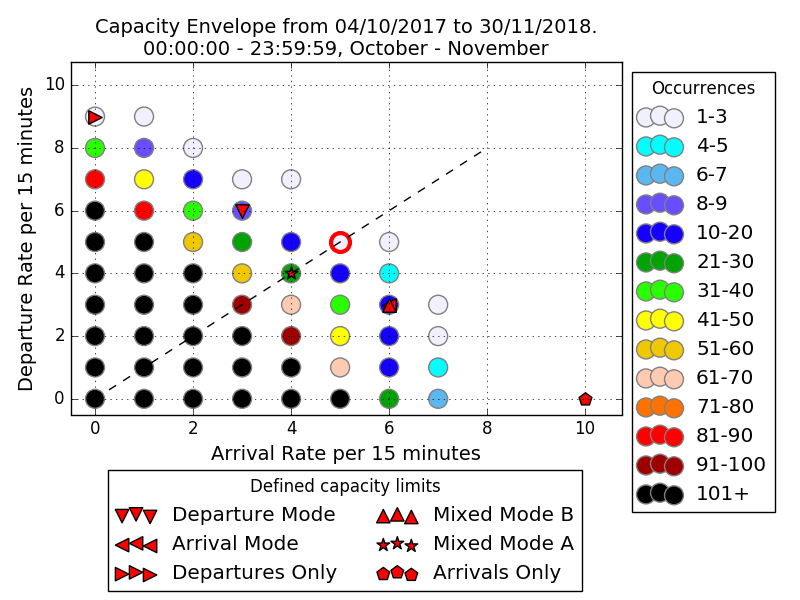
\includegraphics[width=0.8\textwidth]{graphics/fig_Capacity_Envelope_2017-10-04_to_2018-11-30_15min_occurrences_limits.png}
    \caption[Capacity envelope for BIKF]{Capacity envelope at BIKF since October 2017 during peak hours. The measured time interval is 15 minutes and includes both the morning and afternoon peaks. The capacity limits of the airfield are also defined and noted on the figure for various sequence modes. The mixed modes indicate: equal arrivals and departures (Mixed~Mode~A) or two times more arrivals than departures (Mixed Mode B), the latter being a tendency during the afternoon peaks. The figure is from Isavia's internal GUI Víkingaskipið.}  \label{fig:capacity_evnelope}
\end{figure}

This approach indicates a maximum measured capacity of four arrivals to four departures in a "Mixed~Mode~A". This equilibrium mode is defined as the primary measure for the throughput capacity of BIKF. The values are in accord with the defined peak hour intervals in section~\ref{sec:arot_and_study_objective}

There are many aspects of a runway system that can affect the number of aircraft that can land or depart from an airfield and some of those are listed below~\cite{de_neufville_airport_2013, kim_validation_2010}.
\begin{itemize}
    \item Number and geometric layout of the runways.
    \item State and performance of the ATM system.
    \item Wake Separation requirements between aircraft pairs imposed by the ATM.
    \item Weather conditions (visibility, precipitation, cloud ceiling). 
    \item Wind direction and strength.
    \item Mix of aircraft using the airport.
    \item Sequence of movement on each runway (arrivals -- departures split)
    \item Type and location of taxiway exits from the runway.
    \item Runway occupancy time.
    \item Controller workload.
    \item Noise-related constraints and other environmental considerations.
\end{itemize}

Two of the above mentioned factors are principal in determining airfield capacity, namely the wake turbulence separation requirements and runway occupancy time~\cite{kolos2013influence}. Those are in turn influenced by traffic mix, seasonal factors and runway exits, to mention a few. The following Chapter~\ref{cha:methods} on Methods will deal with some of those aspects. 


\section{Wake Turbulence Separation}
This section briefly reviews the necessity of adopting a wake turbulence separation scheme for aircraft from the perspective of fluid dynamics and the overall benefits of the RECAT-EU wake turbulence separation scheme in comparison to the ICAO WTC.

\subsection{Current Understandings of Wake Vortex Behaviour}
Wake vortices describe the nature of the air flow generated behind the wing tips of a jet aircraft~\cite{doc4444full}.
The lift effect on an aircraft wing is created by the differential pressure between the lower and the upper surface of the wing. 
At the wing tips the high pressure flow from the lower side leaks around the tip and to the upper side of the wing. Thus the streamlines over the wing are pushed inwards, while the streamlines under the wing are pushed outwards. When the two streams combine at the trailing edge of a lifting wing, the difference in span-wise velocity causes the air to roll up into a number of small stream-wise vortices distributed along the span of the wing that eventually mix together and are combined into two main counter-rotating vortices aft of the wing as illustrated in Figure~\ref{fig:vortex_develop} ~\cite{houghton2012aerodynamics,magazine_airbus_safety, Breitsamter2011Feb, gerz_commercial_2002}. Between the vortices the induced flow is downwards (downwash) while outside the air moves upwards.

The effect of wake vortices on air masses is known as wake turbulence. 
The kinetic energy contained in the vortices is dependent on the weight and aerodynamics of the generating aircraft. The cross flow velocities in the core region of the trailing vortices can reach $360$ km/h and the vortices can stay effective up to hundred wing spans, which can result in wake vortices lasting for several minutes and up to $30$ km behind larger aircraft~\cite{Breitsamter2011Feb, gerz_commercial_2002}. 
\begin{figure}[h]
    \centering
    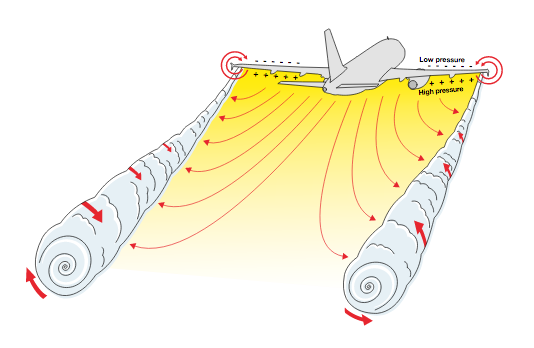
\includegraphics[width=0.8\textwidth]{graphics/WakeVortexPlane.png}
    \caption[Wake vortex roll-up process]{Wing vortex evolution and roll-up process. Two main vortices form behind the aircraft turning in opposite directions, clockwise behind the left wing (seen from behind) and anti-clockwise behind the right one~\cite[p.~043]{magazine_airbus_safety}} \label{fig:vortex_develop}
\end{figure}

\subsection{Ground Effect and Vortex Decay Rate}
Wake vortices tend to descend slowly to an altitude of about one half of the initial separation, near ground on approach for landing.
Upon reaching this point the descent will stop and then ascend slowly. This "re-bounce" effect is caused by the presence of the ground and carries with it the formation of a second pair of induced vortices outside and below the main vortex. 

In the presence of stable cross-wind conditions the decay of the downwind vortex is not identical to the upwind vortex and the descent rate may vary significantly~\cite{Hallock2018Apr}. 
The trajectories of the vortex pair may be modified and the upwind vortex could stall over the runway while the downwind vortex ascends and decays faster (Figure~\ref{fig:vortex_ground_effect}).
\begin{figure}[h]
    \centering
    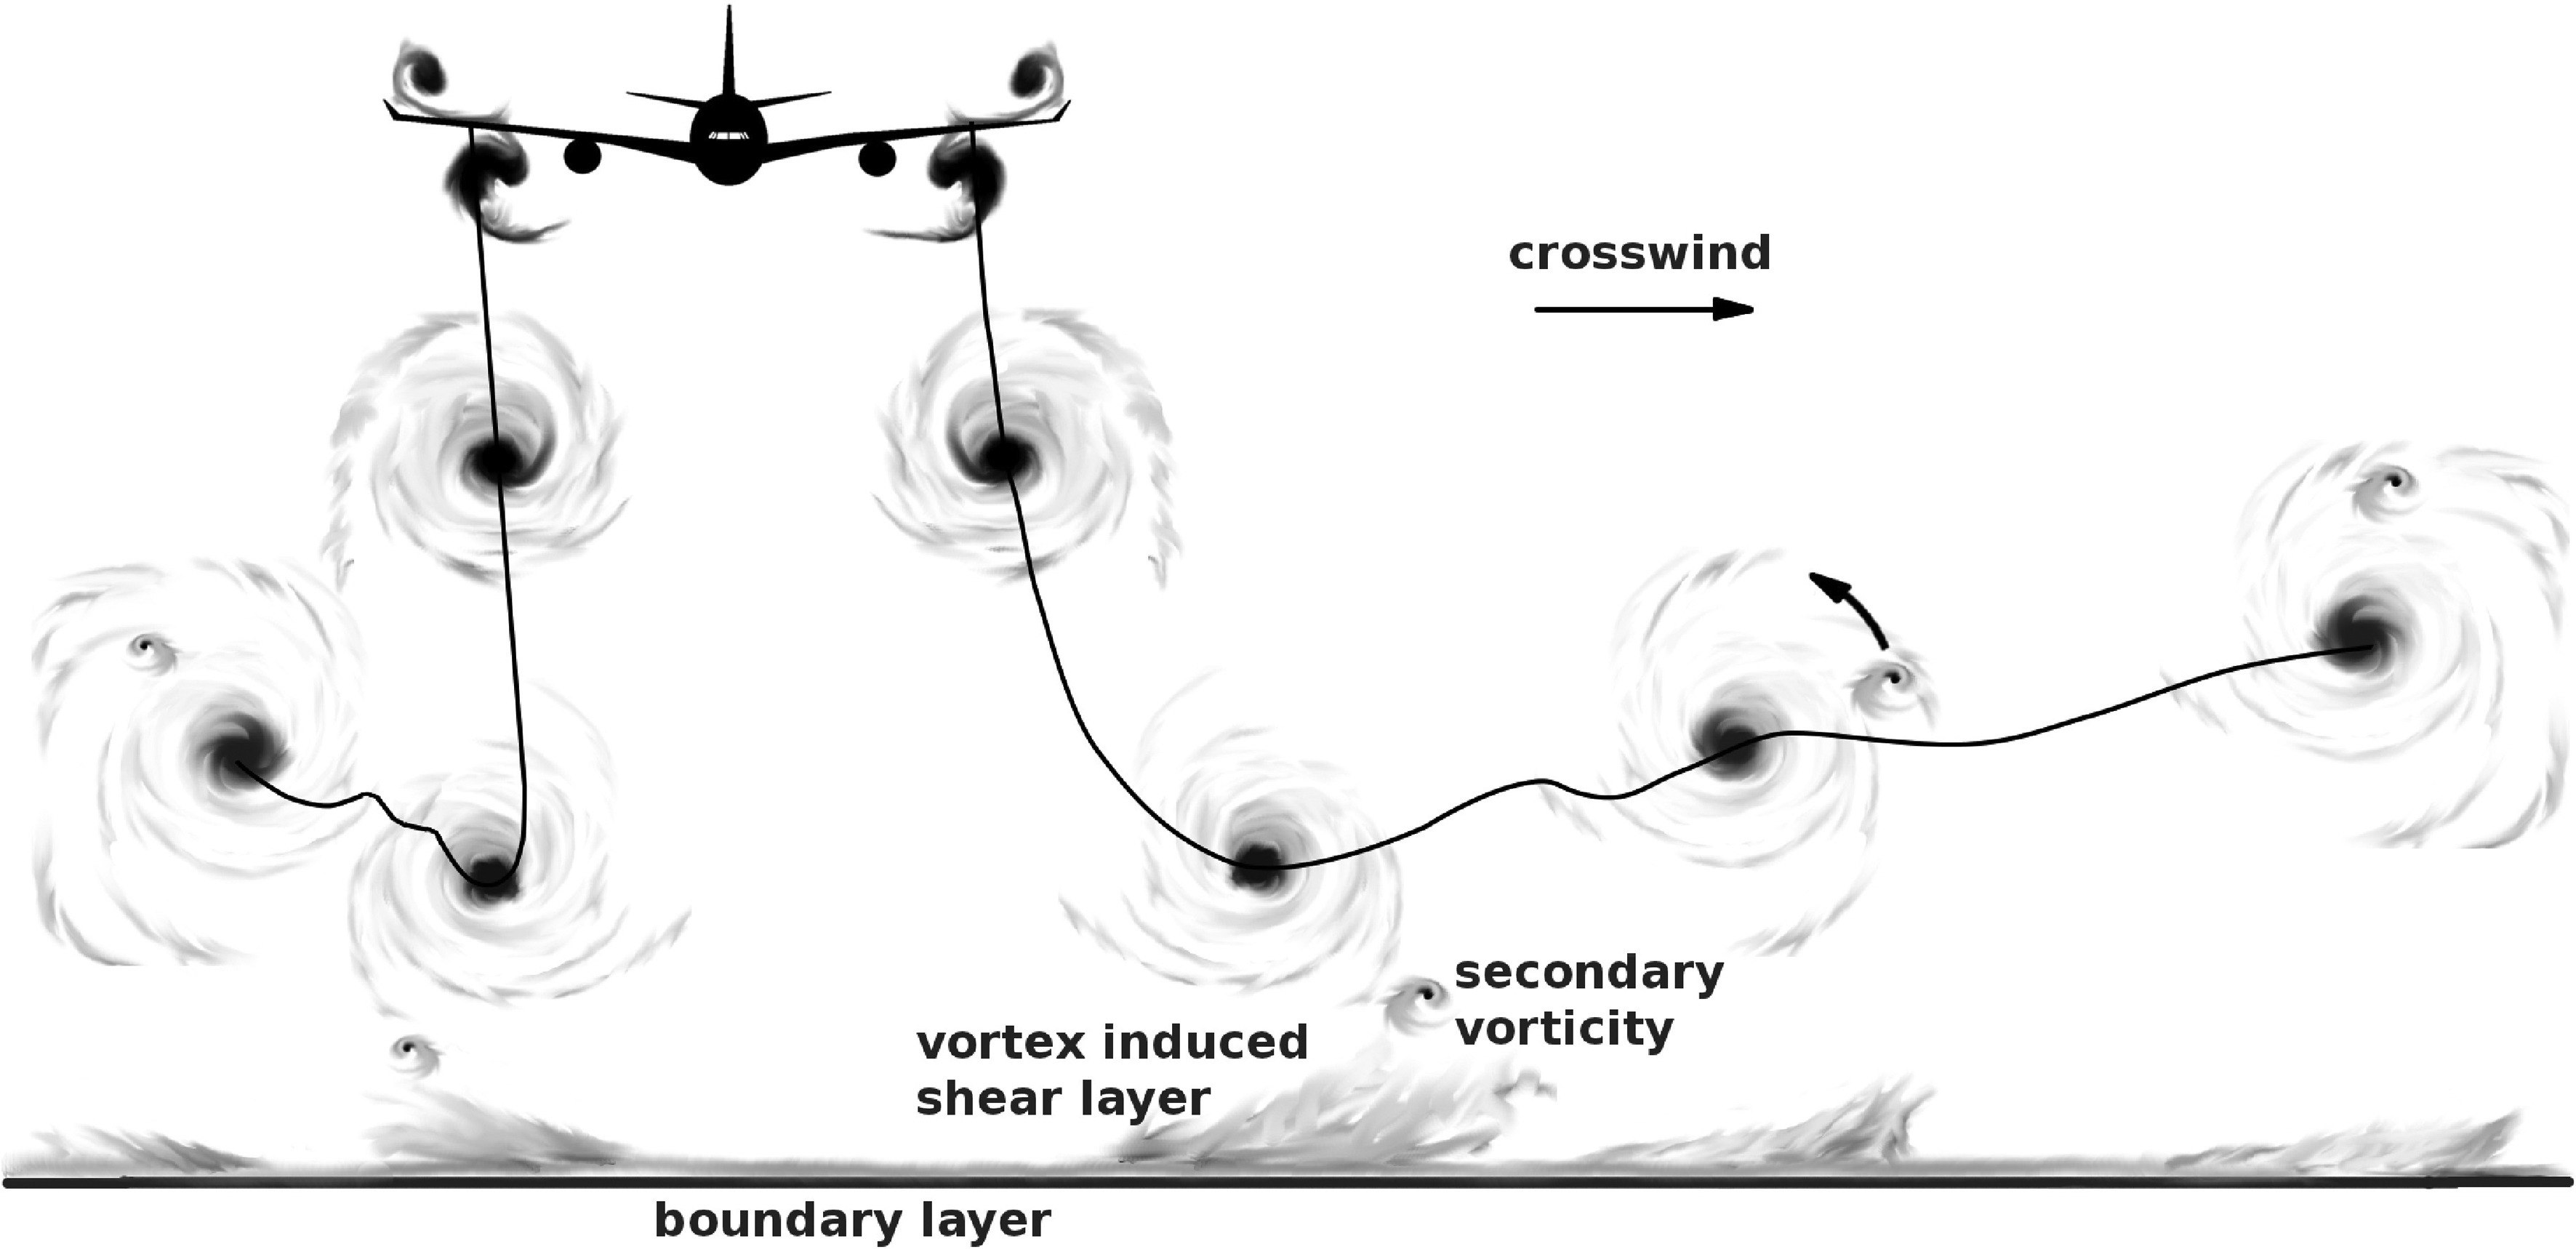
\includegraphics[width=0.8\textwidth]{graphics/Hallock_vortex_evolution.jpg}
    \caption[Wake vortex and ground effect]{Vortex evolution and ground effect~\cite[p.~29]{Hallock2018Apr}.} \label{fig:vortex_ground_effect}
\end{figure}

Measurements have shown that the lateral/sideways motion of a vortex in an airport environment could range between $229$~m and $518$~m and in some cases even $762$~m, which is the basis for the "2500-foot" rule separation in parallel runway configurations~\cite{Hallock2018Apr, hallock2004summary, hallock2003wake}.
The vertical descent rate of vortices for medium commercial aircraft in stable atmosphere is shown to be around $1.5-2.5$~m/s for the first $30$~seconds after which the descent slows and eventually approaches zero at $152-274$ m below the flight path, and for heavier aircraft decaying vortices have been observed at $305$~m below of the flight path~\cite{lissaman1973aircraft, Hallock2018Apr}. 

Aerodynamic properties of the aircraft govern the vortex roll-up process and ambient atmospheric conditions dominate the behaviour of the vortices forcing instability and eventual decay of the vortices~\cite{Hallock2018Apr}.
Several factors that drive the decay rate of the vortex pair have been formulated:
\begin{itemize}
    \item Atmospheric turbulence extracts energy from the vortex and reduces its strength leading to a faster wake decay ~\cite{Hallock2018Apr}.
    \item Viscosity of the atmosphere also draws out energy from the vortex but at a slower rate than the atmospheric turbulence. The so called dissipative action of viscosity  effectively removes energy from a disturbance, in this case a vortex, thereby causing it to decay~\cite{Hallock2018Apr, houghton2012aerodynamics}.
    \item Buoyancy force acts on the vortex in a thermally stable stratified environment as a result of the lesser air density inside the vortex system and may causes stall or rebound to the flight level~\cite{Holzapfel2001Feb, gerz_commercial_2002}.
    \item Vortex instability in the form of long wave sinusoidal fluctuations of the vortex core (Crow instability) may occur due to light turbulence in the atmosphere and may cause the vortices to link and decay faster~\cite{dup._donamdson_vortex_1975, Hallock2018Apr, crow2003stability}.
    \item Secondary vorticity structures, vertical rib-like counter rotating flow formations may appear between the vortex pair and eventually wrap around the main vortices, leading to turbulence build inside the system and rapid circulation decay~\cite{Holzapfel2001Feb, Holzapfel2003Jun}.
\end{itemize}

Wake vortex characteristics of conventional aircraft have been studied for several decades now and "it is generally acknowledged that the near wake of a large jet airliner poses a significant hazard to any smaller aircraft that follows it into of out of an air terminal"~\cite[p.~5]{dup._donamdson_vortex_1975}.

Distance separation between aircraft is necessary to mitigate the effect of the wake vortices. This is especially true for aircraft in approach for landing or take-off, "since practically all serious problems associated with wake hazard occur in the vicinity of airports"~\cite[p.~5]{dup._donamdson_vortex_1975}. 
The wake vortices generated by a leading aircraft (leader) can cause loss of lift or an induced rolling moment and velocity fluctuations in a following aircraft (follower), if the follower enters the wake turbulence region near the leader~(Figure~\ref{fig:vortex_encounter}).

\begin{figure}[h]
    \centering
    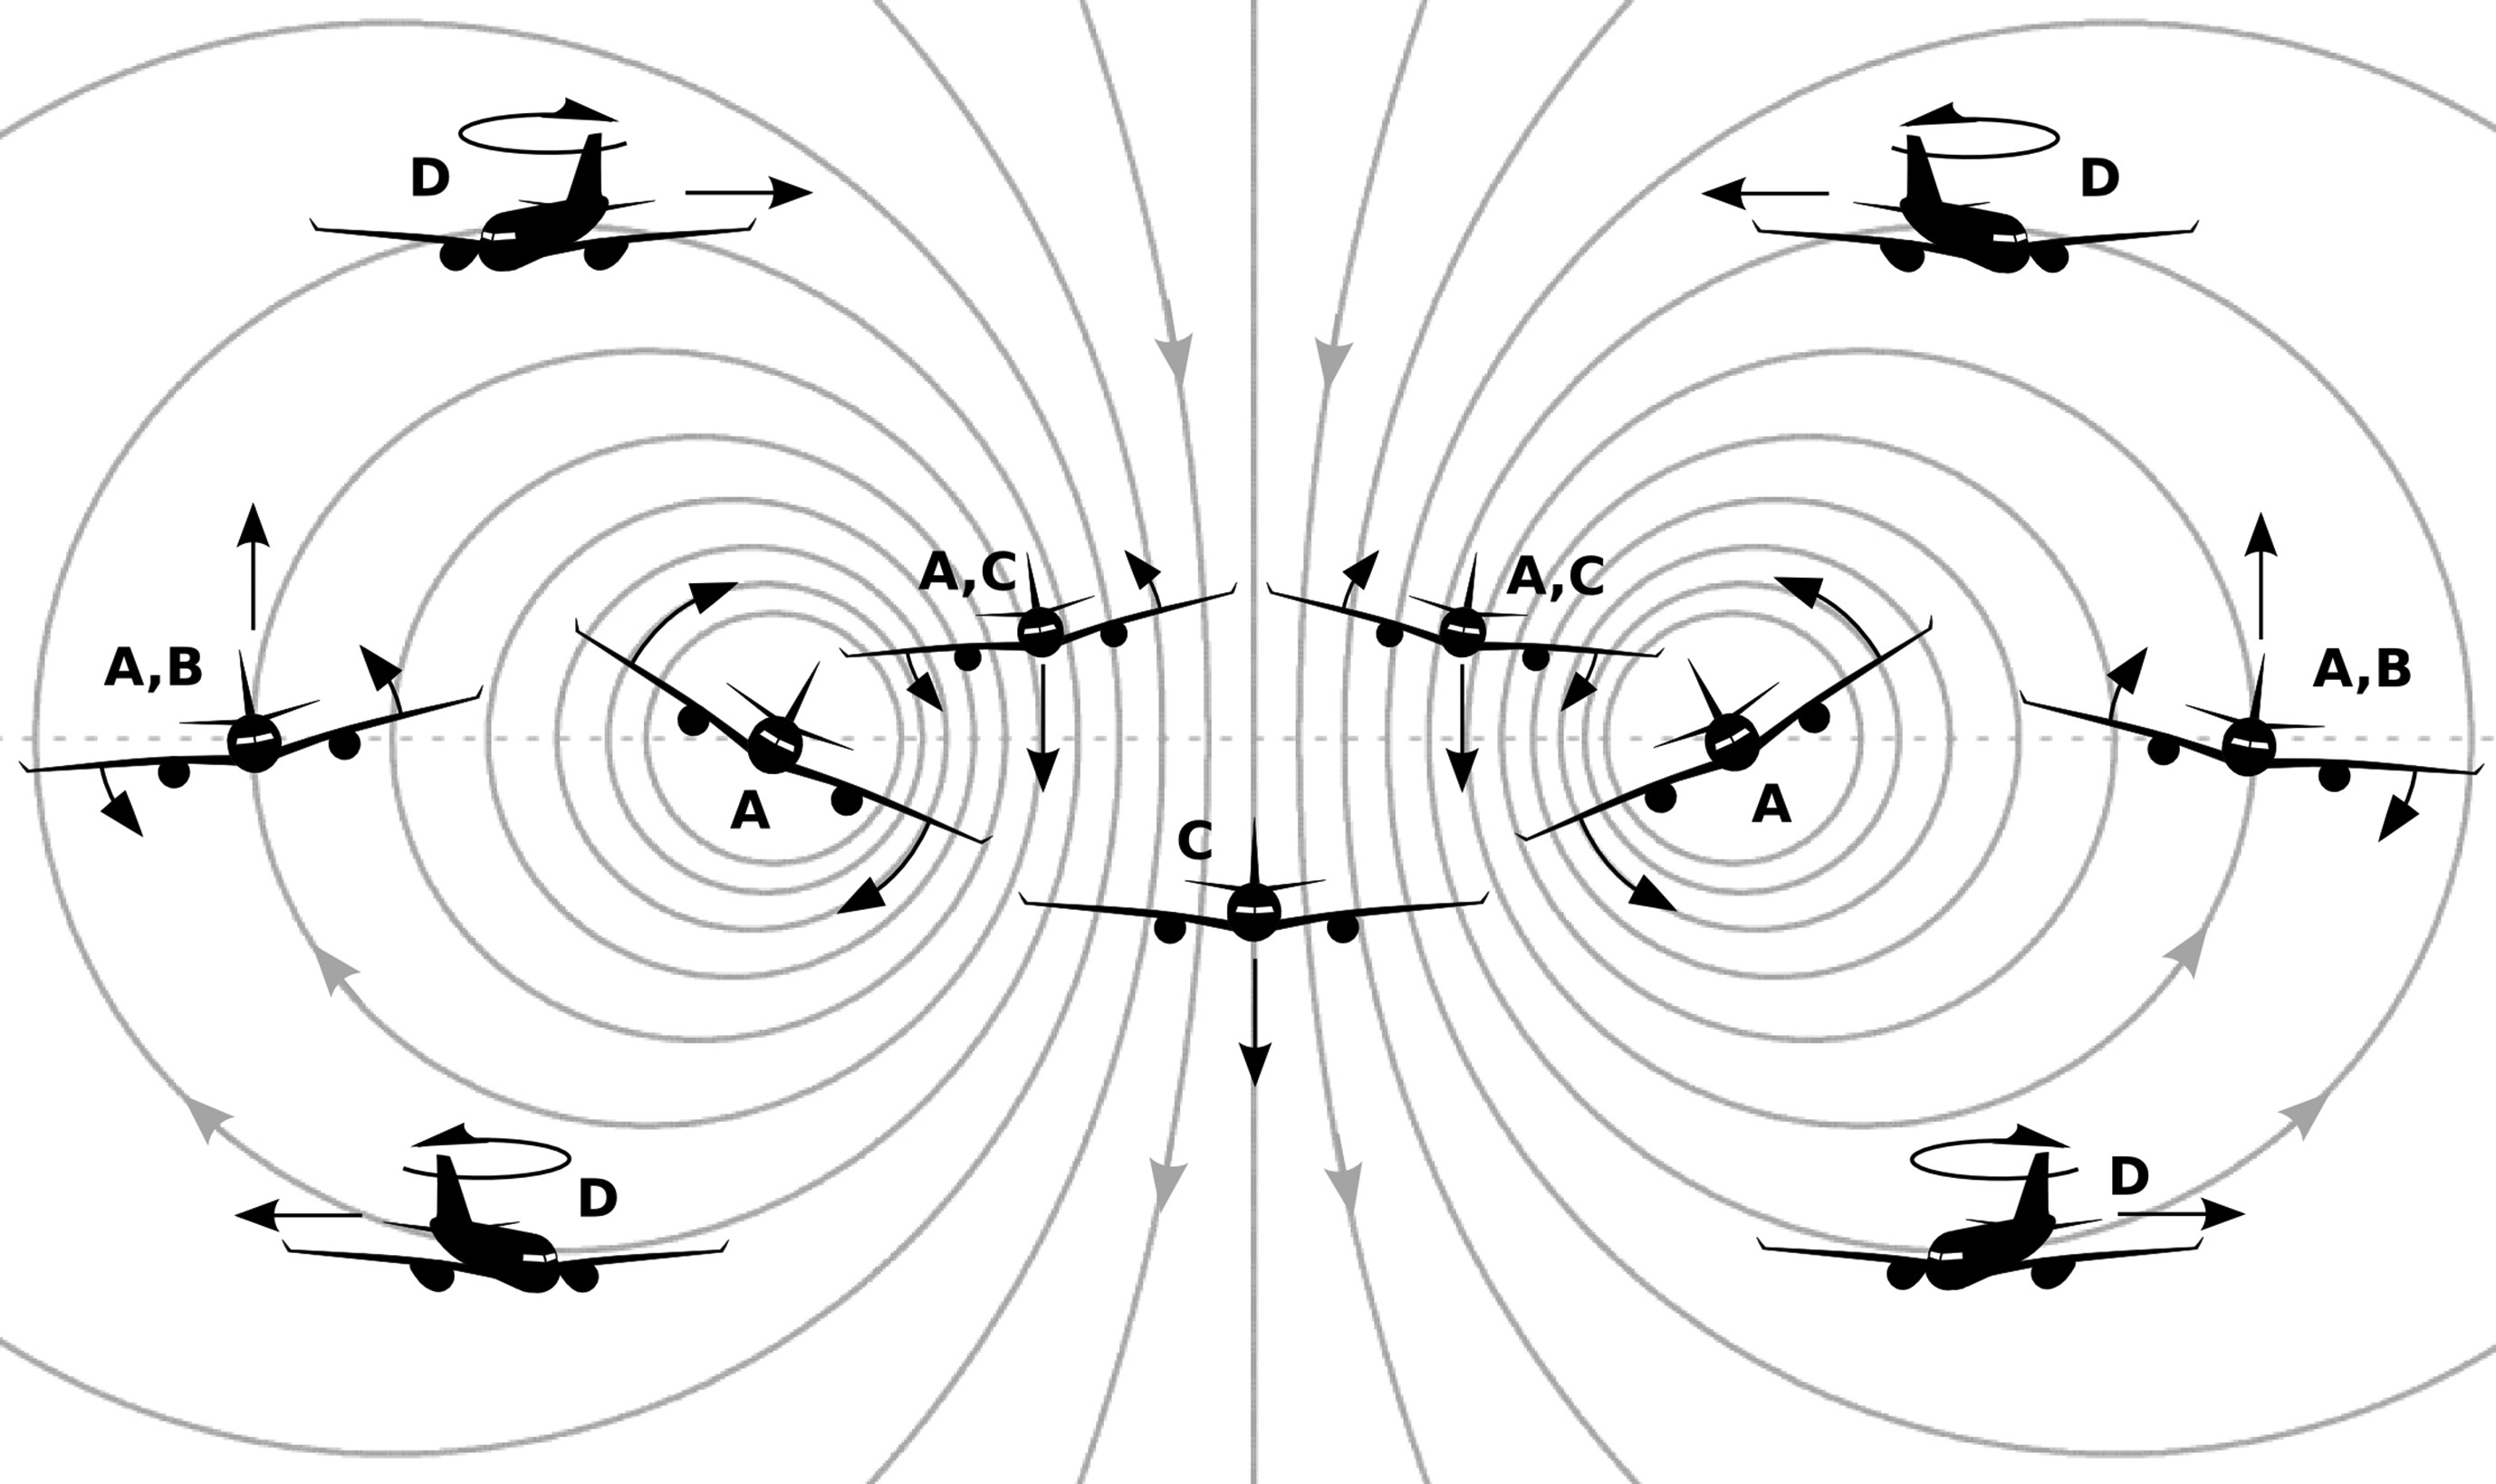
\includegraphics[width=0.8\textwidth]{graphics/reaction_in_wake.jpg}
    \caption[Wake vortex encounter]{Effect of wake vortex flow field on an aircraft: induced rolling moment (A), upward motion (B), loss of lift (C), yaw motion (D)~\cite[p.~33]{Hallock2018Apr}} 
    \label{fig:vortex_encounter}
\end{figure}

This can lead to the up-set and potentially loss of control of an aircraft following the flight path of a preceding aircraft.
To diminish the effect of such vortices the trailing aircraft must be maintained at a safe distance behind the leading aircraft as the vortices spread laterally to either side of the flight path and are dissipated~\cite{Breitsamter2011Feb}.
The distance between aircraft pairs in view of safety is referred to as wake vortex separation. 

\subsection{Wake Turbulence Categorisation}
Traditional separation standards, introduced in the 1970s, are defined by ICAO based on certificated Maximum Take-Off Mass (MTOM) of aircraft. The MTOM criteria allocates each aircraft in a wake turbulence category. The prescribed categories are three i.e. Heavy, Medium and Light.
The Heavy category includes aircraft with MTOM larger than $136.000$~kg. The aircraft in the Medium category have MTOM between $7.000$~and~$136.000$~kg and the Light category includes the aircraft with maximum take-off mass less than or equal to $7.000$~kg.
In addition, for aircraft in the order of $560.000$~kg, ICAO provides a subcategory to the Heavy types called Super Heavy (Table~\ref{tab:WTC}). 

\begin{table}[ht]
    \centering
    \resizebox{1\textwidth}{!} {
    \begin{tabular}{l|c|c|c|c|c|c}
    ~    & \multicolumn{6}{c}{Category} \\ \hline
    ICAO & Super Heavy & Heavy (H) & \multicolumn{2}{c|}{Medium (M)} & \multicolumn{2}{c}{Light (L)} \\
    
    ~    & A380-800    & > 136.000  & \multicolumn{2}{c|}{ 136.000 -- 7.000 } & \multicolumn{2}{c}{$ \leq 7.000$} \\ \hline
    
    ICAO (UK)   & ~  & Heavy (H) & Upper Medium (UM) & Lower Medium (LM) & Small (S)  & Light (L) \\
    
    ~    & A380-800    & > 136.000  & 136.000 -- 104.000     & 104.000 -- 40.000      & 40.000 -- 17.000 & $ \leq 17.000 $   \\ \hline
    
    FAA (US)   & Super      & Heavy & B757   & Large   & \multicolumn{2}{c}{Small} \\
    
    ~    & A380        &  > 136.000   & ~                 &  136.000 -- 18.600       & \multicolumn{2}{c}{$ \leq 18.600 $} \\ 
    \end{tabular}}
    \caption[ICAO wake turbulence categories based on maximum take-off mass]{ICAO wake turbulence categories of transport aircraft based on maximum take-off mass (MTOM) in~kg~\cite{doc4444full, uk_aeronautical_information_services_wake_2017, kolos2013influence}.} \label{tab:WTC}
\end{table}

Some countries have chosen to further increase the number of the ICAO wake turbulence categories in light of safe airport operational experience. Aerodromes in the UK split the Medium and Light categories each into two subcategories (Table~\ref{tab:WTC}), while the Federal Aviation Administration (FAA) places Boeing~B757 into a separate category and increases the upper weight limit of the Small (Light) category to $18.600$~kg. The Boeing~757s are known to generate unusually high core vortex speed.~\cite{icao_wtc, uk_aeronautical_information_services_wake_2017, noauthor_recat_2018}

Under standard ICAO criteria, each aircraft is allocated in a wake category and the categories form pairs: a combination of a leader and a follower aircraft. Each pair is assigned a distance separation minima, depending on the wake turbulence generated by the leader and applied to the follower. Conventionally the separations are expressed in Nautical Miles (NM). The leader-follower combinations can be charted as a wake turbulence separation matrix~(Table~\ref{tab:ICAO_WTC}), in which the elements indicate the minimum spacing for each pair.

% Please add the following required packages to your document preamble:
% \usepackage{multirow}
% \usepackage{graphicx}
\begin{table}[h]
\centering
\resizebox{.8\textwidth}{!}{%
\begin{tabular}{|c|c|c|c|c|c|}
\hline
\multicolumn{2}{|c|}{\multirow{2}{*}{ICAO WTC scheme}} & \multicolumn{4}{c|}{Follower}              \\ \cline{3-6} 
\multicolumn{2}{|c|}{}                                 & Super (A380-800) & Heavy & Medium & Light \\ \hline
\multirow{4}{*}{\rotatebox[origin=c]{90}{Leader}}       & Super (A380-800)       & (*)                & 6 NM  & 7 NM   & 8 NM   \\ \cline{2-6} 
                              & Heavy                  & (*)                & 4 NM  & 5 NM   & 6 NM   \\ \cline{2-6} 
                              & Medium                 & (*)                & (*)     & (*)      & 5 NM   \\ \cline{2-6} 
                              & Light                  & (*)                & (*)     & (*)      & (*)      \\ \hline
\end{tabular}%
}
\caption[ICAO wake turbulence categories and separation minima]{ICAO wake turbulence categories and separation minima to avoid wake vortex encounter.(*) indicate Radar Separation Minimum (MRS)~\cite{noauthor_recat_2018, rooseleer2015recat}.} \label{tab:ICAO_WTC}
\end{table}

The wake turbulence separation must be observed, for arrival and departure, when the airport operates under Instrument Flight Rules (IFR). The IFR allow properly equipped aircraft to be flown under impaired visibility conditions. When Visual Flight Rules (VFR) are in effect (flight visibility 5 km, clear of clouds and in sight of the surface), the separation may be decided by the pilot within observed safety limits.~\cite{gerz_commercial_2002, icao_annex_2005} 

When wake turbulence separation requirements are not specified and a surveillance system like radar is used, the longitudinal separation minimum may be reduced by the Air Traffic Management (ATM), if the surveillance system's capabilities at a given location permit this~\cite{MRS_separation_standard}. The Radar Separation Minimum (MRS) for aircraft established on the same final approach track is 3~NM (or 2,5~NM under given conditions) as prescribed by ICAO Doc 4444 PANS-AM~\cite{doc44444}.

\begin{figure}[h]
    \centering
    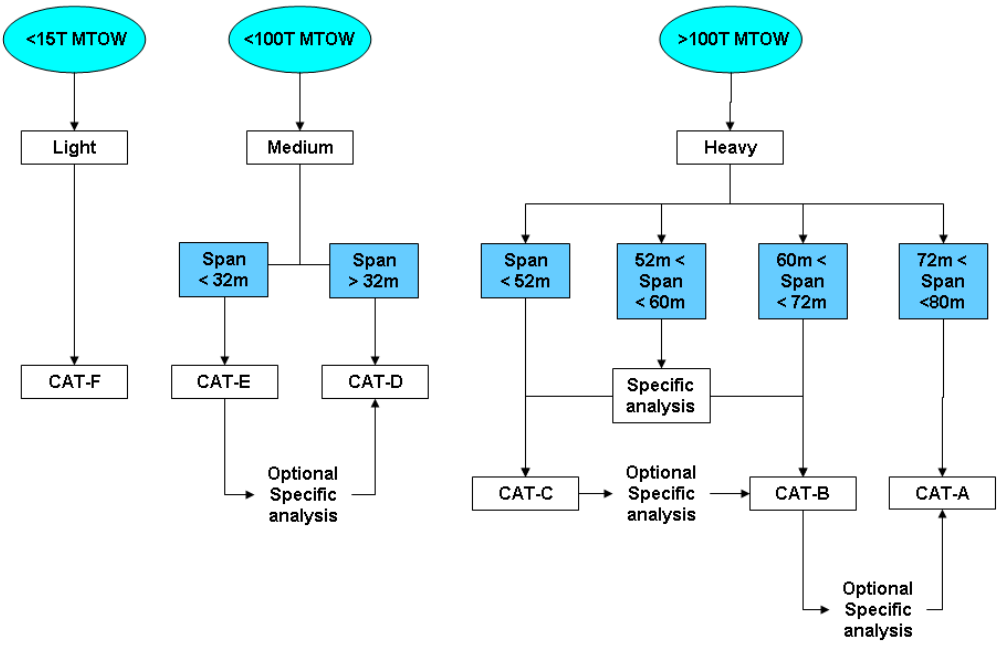
\includegraphics[width=1\textwidth]{graphics/Criteria_RECAT.png}
    \caption[RECAT-EU categorisation criteria]{Categorisation process and criteria for assigning an existing aircraft type into RECAT-EU scheme~\cite[p.~15]{rooseleer2015recat}} \label{fig:RECAT_criteria}
\end{figure}

The ICAO wake turbulence separation rules outline the "worst case" for each category and thus generate over-separation in many cases~\cite{noauthor_recat_2018, rooseleer2015recat}. The categorisation was implemented over 40 years ago and has become out-of-date in view of the newer aircraft models. Consequently EUROCONTROL has developed the European Wake Vortex Re-categorisation (RECAT-EU) as a more precise categorisation of aircraft compared to ICAO WTC. The objective was to safely help increase airport capacity and reduce delays by redefining wake turbulence categories and their associated separation 
minima. RECAT-EU is based on the ICAO scheme and takes into account Maximum Take-Off Weight (MTOW) and the wing span of the aircraft (Figure~\ref{fig:RECAT_criteria}).

According to EUROCONTROL the expected immediate benefits from RECAT-EU deployment are: increased runway throughput around 5\% and operational efficiency during peak periods. The runway capacity increase with RECAT-EU "comes from the categorisation and separation reduction for aircraft types which are predominant in European traffic"~\cite[p.~22]{rooseleer2015recat}. Implementation of RECAT-EU will mean a minimum ATM system update and does not require deployment of new technologies.

The resulting categories following the re-categorisation criteria from Figure~\ref{fig:RECAT_criteria} are six:

\begin{tabular}{l}
    \textbullet \space CAT A -- "Super Heavy" \\
    \textbullet \space CAT B -- "Upper Heavy"\\
    \textbullet \space CAT C -- "Lower Heavy"\\
    \textbullet \space CAT D -- "Upper Medium"\\
    \textbullet \space CAT E -- "Lower Medium"\\
    \textbullet \space CAT F -- "Light"\\ 
\end{tabular}

The RECAT-EU wake turbulence separation matrix combining leader and follower into pairs with assigned minimum spacing for each pair is shown in Table~\ref{tab:RECAT-dist}. The application of instrumental or visual flight rules and the MRS procedures remain identical to the ICAO WTC scheme. The introduction of RECAT-EU alters only the spacing between 
certain aircraft in a pair, which is applied to arrivals as well as departures.

\begin{table}[h]
\centering
\resizebox{.8\textwidth}{!}{%
\begin{tabular}{|c|c|c|c|c|c|c|c|}
\hline
\multicolumn{2}{|c|}{\multirow{2}{*}{RECAT-EU scheme}} & \multicolumn{6}{c|}{Follower}                   \\ \cline{3-8} 
\multicolumn{2}{|c|}{}                                 & CAT-A & CAT-B & CAT-C & CAT-D & CAT-E & CAT-F \\ \hline
\multirow{6}{*}{\rotatebox[origin=c]{90}{Leader}}            & CAT-A            & 3 NM   & 4 NM  & 5 NM  & 5 NM  & 6 NM  & 8 NM  \\ \cline{2-8} 
                                    & CAT-B            &    (*)    & 3 NM  & 4 NM  & 4 NM  & 5 NM  & 7 NM  \\ \cline{2-8} 
                                    & CAT-C            &    (*)    & (*)   & 3 NM  & 3 NM  & 4 NM  & 6 NM  \\ \cline{2-8} 
                                    & CAT-D            &    (*)    &   (*)    &    (*)   &   (*)    &   (*)    & 5 NM  \\ \cline{2-8} 
                                    & CAT-E            &    (*)    &   (*)    &   (*)    &   (*)    &   (*)    & 4 NM  \\ \cline{2-8} 
                                    & CAT-F            &    (*)    &   (*)    &    (*)   &   (*)    &   (*)    & 3 NM  \\ \hline
\end{tabular}%
}
\caption[RECAT-EU distance-based separation minima]{RECAT-EU wake turbulence distance-based separation minima on approach and departure. (*) indicates minimum radar separation (MRS), set at 3~NM (2,5~NM under given conditions), applicable as per current ICAO doc 4444 provisions \cite{doc44444, rooseleer2015recat, noauthor_recat_2018}.}
\label{tab:RECAT-dist}
\end{table}

The noticeable changes in wake turbulence separation under RECAT-EU from ICAO WTC are systematised in Table~\ref{tab:delta_distance_wtc2recat}. A beneficial change in wake turbulence separation experiences for example a Heavy leader -- Medium follower aircraft pair, which after re-categorisation form a CAT-C -- CAT-D pair. In this case, the separation from the leader can be reduced by up to 2~NM. 

\begin{table}[h]
\centering
\resizebox{.9\textwidth}{!}{%
\begin{tabular}{|c|c|c|c|c|c|c|c|}
\hline
\multicolumn{2}{|c|}{}                                          & \multicolumn{6}{c|}{Follower}                                                                                                                                                                                                   \\ \cline{3-8} 
\multicolumn{2}{|c|}{\multirow{-2}{*}{RECAT-EU scheme}} & CAT-A                             & CAT-B                                & CAT-C                         & CAT-D                         & CAT-E                         & CAT-F                                                \\ \hline
                                                        & CAT-A & \cellcolor[HTML]{FD6864}(+0,5 NM) & \cellcolor[HTML]{67FD9A}-2 NM        & \cellcolor[HTML]{67FD9A}-1 NM & \cellcolor[HTML]{67FD9A}-2 NM & \cellcolor[HTML]{67FD9A}-1 NM &                                                      \\ \cline{2-8} 
                                                        & CAT-B &                                   & \cellcolor[HTML]{67FD9A}-1 NM        &                               & \cellcolor[HTML]{67FD9A}-1 NM &                               & \cellcolor[HTML]{FD6864}+1 NM                        \\ \cline{2-8} 
                                                        & CAT-C &                                   & \cellcolor[HTML]{67FD9A}-1 (-1,5) NM & \cellcolor[HTML]{67FD9A}-1 NM & \cellcolor[HTML]{67FD9A}-2 NM & \cellcolor[HTML]{67FD9A}-1 NM &                                                      \\ \cline{2-8} 
                                                        & CAT-D &                                   &                                      &                               &                               &                               &                                                      \\ \cline{2-8} 
                                                        & CAT-E &                                   &                                      &                               &                               &                               & \cellcolor[HTML]{67FD9A}{\color[HTML]{000000} -1 NM} \\ \cline{2-8} 
\multirow{-6}{*}{\rotatebox[origin=c]{90}{Leader}}                                & CAT-F &                                   &                                      &                               &                               &                               & \cellcolor[HTML]{FD6864}(+0,5 NM)                    \\ \hline 
\end{tabular}%
}
\caption[Difference in wake turbulence separation minima between ICAO and RECAT-EU schemes]{Difference in wake turbulence separation minima on approach between reference ICAO and RECAT-EU schemes (full proposal)~\cite{rooseleer2015recat}}
\label{tab:delta_distance_wtc2recat}
\end{table}

The different category code names in this study will be referred to on a single letter basis for simplification e.g. "CAT-C" will be abbreviated to "C", "CAT-D" to "D", "Heavy" to "H", Medium to "M" and so forth. This applies to pair categories as well by abbreviating e.g. "CAT-C leader -- CAT-D follower"  to "C-D pair" or just "C-D", and "Medium--Medium" pair to "M-M".

\section{Arrival Runway Occupancy Time and Landing Time Interval}\label{sec:arot_and_study_objective}

The Runway Occupancy Time (ROT) is defined by EUROCONTROL as the length of time that each aircraft occupies the runway~\cite{ROT_definition}. 
This project focuses on Arrival Runway Occupancy Time (AROT) during peak traffic hours, that is the time interval defined by an aircraft crossing the threshold and its tail vacating the runway~\cite{AROT_definition}. The threshold is the beginning of that portion of the runway that is available for landing.

The peak traffic hours are characterised by the time intervals when the airport operates at high loads. High load interval or window is at least 15 minutes in length and has five or more flights arriving or departing from Keflavík Airport. The time between flights during the high load interval is set at $\leq$4~minutes (Figure~\ref{fig:Peak_Diagram}). This value is based on statistical estimations by Isavia in order to achieve two distinct peak hours: one in the morning and one in the afternoon. The last flight in a high load window that fulfils these requirements is not considered to be a part of the peak as its behaviour is not affected by an instantaneous next flight after it. 

\begin{figure}[h]
    \centering
    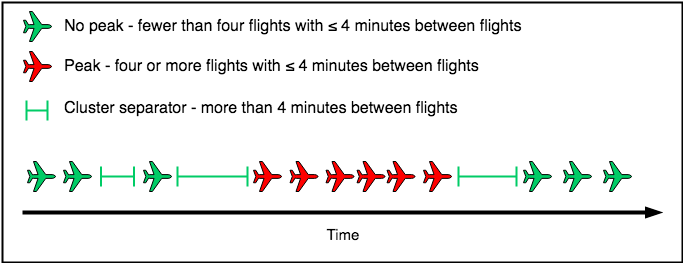
\includegraphics[width=1\textwidth]{graphics/Peak_Diagram.png}
    \caption[Rules defining a peak hour]{Rules used by Isavia to identify a high load interval as peak or not. The time separating each two aircraft in a peak cluster (red) is set as less than or equal to 4 minutes. The last red aircraft in the peak cluster is not counted as part of the peak. Cluster separators are defined as time intervals larger than four minutes.}
    \label{fig:Peak_Diagram}
\end{figure}

The AROT metric is essential for the project because a following aircraft is not allowed to land on the same runway before it has been vacated by the leading aircraft. The interval to the next landing aircraft is specified as the Landing Time Interval (LTI) which is directly linked to the inter-arrival distance or in other words the wake turbulence separation. The LTI is a metric used to quantify the time separation between aircraft in a pair, derived from the distance separation between the aircraft and the final approach speed of the following aircraft. One way the conflict between the AROT and LTI can manifest itself is through a missed approach (ICAO: bulked landing), when an aircraft landing cannot be completed due to runway incursion \cite{doc44444}: the incorrect presence of another aircraft on the runway designated for landing.% (time travelled is distance travelled divided by velocity).

The goal of examining the arrival runway occupancy times and the landing time intervals is to determine whether the implementation of the RECAT-EU scheme at BIKF under certain conditions, would affect the throughput of the airfield. Additionally the analysis could indicate whether the limiting factor is the runway occupancy time or the separation requirement. The proposed transition by EUROCONTROL from ICAO WTS to RECAT-EU scheme suggests reduced distance separation for certain aircraft pairs (Table~\ref{tab:delta_distance_wtc2recat}). This reduction, revealed by shifting the wake turbulence separation minima for arrival pairs, creates potential for reduced spacing between aircraft, hence reducing the time interval between landings (LTI) and facilitating increased throughput capacity of the runways. 

\begin{figure}[h]
    \centering
    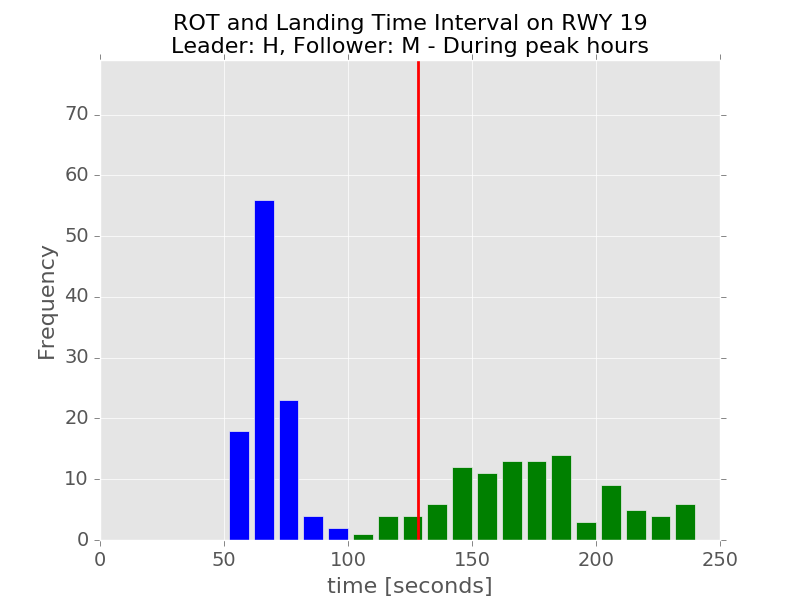
\includegraphics[width=0.8\textwidth]{graphics/fig_rot_landig_time_interval_RWY19_leader_H_follower_M_peak-hour_BAR_20171004_20181130.png}
    \caption[AROT and LTI of H-M pairs on RWY~19]{Arrival runway occupancy time (blue) and landing time intervals (green) for Heavy leader - Medium follower pairs on BIKF runway RWY-19. The observed time period is from October 2017 to November 2018. The red line indicates the ICAO WTC reference time separation for the selected H-M aircraft pairs. The figure is from the Isavia's internal GUI Víkingaskipið.}\label{fig:AROT_LTI_rwy19_H_M}
\end{figure}

The hypothesis may be illustrated with Figure~\ref{fig:AROT_LTI_rwy19_H_M}. The current ICAO time reference separation, indicated by the red vertical line for BIKF RWY-19 will be relocated to the left for some of the aircraft pairs under the RECAT-EU scheme, following a decreased wake separation requirement. This relocation will be more noticeable for C-C and C-D pairs formed from the ICAO H-M pairs, in which case the separation is reduced from 5~NM to 3~NM. A shift of the reference separation line creates the potential for a shift in the distribution of the LTI, as long as it does not overlap with the AROT. Furthermore, study on the runway capacity of significantly larger airports~\cite{kolos2013influence} suggests that the frequency distribution of LTI tends to compress or squeeze to the right of the reference line with less standard deviation about the mean when the air traffic is intensified.






%%% Local Variables: 
%%% mode: latex
%%% TeX-master: "DEGREE-NAME-YEAR"
%%% End: 
